% ============================================================
% C093: 共焦椭圆与双曲线公共点的焦半径公式
% 与上传原模板一致：\Conclusion + 六个 box 内容文件的 \input 入口
% 图文件新增于 assets/tikz/；不改动现有其他编号的 TikZ 图
% ============================================================
\Conclusion
\subsection{C093 共焦椭圆与双曲线公共点的焦半径公式}
\begin{statementbox}
\textbf{C093\quad 共焦椭圆与双曲线公共点的焦半径公式}

\textbf{条件：}左、右焦点分别是 $F_1=(-c,0)$、$F_2=(c,0)$，$c>0$。
椭圆 $E$ 使用小写半轴 $a,b$，双曲线 $H$ 使用大写半轴 $A,B$，
两曲线标准方程分别为
\[
\boxed{E:\ \frac{x^2}{a^2}+\frac{y^2}{b^2}=1},\qquad
\boxed{H:\ \frac{x^2}{A^2}-\frac{y^2}{B^2}=1}.
\]
其中
\[
a>b>0,\quad A>0,\ B>0,\qquad
a^2-b^2=A^2+B^2=c^2,\quad c>0.
\]
因此 $a>c>A>0$。点 $P=(x_P,y_P)$ \emph{同时在 $E$ 和 $H$ 上}。

\begin{center}
% C093: a=4, A=1, c=2; E: x^2/16+y^2/12=1, H: x^2-y^2/3=1
% Intersection P=(2,3); PF1=5, PF2=3; generated as exact coordinate constructions.
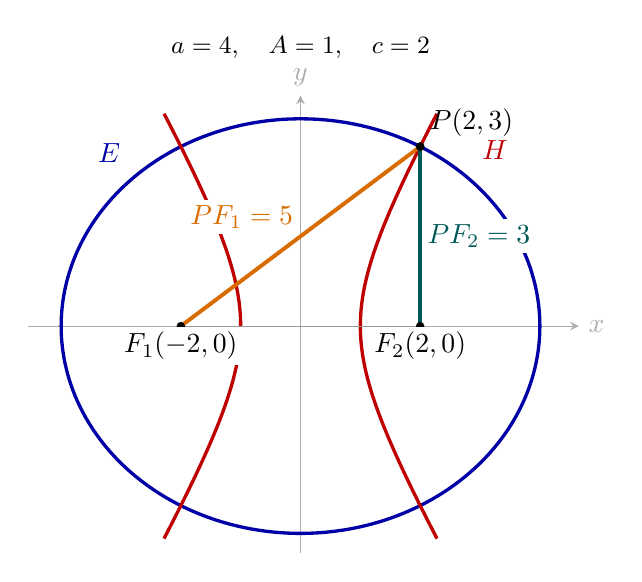
\begin{tikzpicture}[scale=0.76,>=stealth]
 \node[font=\small] at (0,4.65) {$a=4,\quad A=1,\quad c=2$};
 \draw[->,gray!65] (-4.55,0)--(4.65,0) node[right]{$x$};
 \draw[->,gray!65] (0,-3.8)--(0,3.85) node[above]{$y$};
 \draw[blue!65!black,very thick,samples=160,domain=0:360,smooth,variable=\t]
  plot ({4*cos(\t)},{sqrt(12)*sin(\t)});
 \draw[red!75!black,very thick,samples=110,domain=-3.55:3.55,variable=\t]
  plot ({sqrt(1+\t*\t/3)},{\t});
 \draw[red!75!black,very thick,samples=110,domain=-3.55:3.55,variable=\t]
  plot ({-sqrt(1+\t*\t/3)},{\t});
 \coordinate (L) at (-2,0); \coordinate (R) at (2,0); \coordinate (P) at (2,3);
 \draw[orange!85!black,line width=1.4pt] (L)--(P) node[midway,above left,fill=white,inner sep=2pt]{$PF_1=5$};
 \draw[teal!70!black,line width=1.4pt] (R)--(P) node[midway,right,fill=white,inner sep=2pt]{$PF_2=3$};
 \draw[gray!80] (L)--(R);
 \fill (L) circle (2pt) node[below,fill=white,inner sep=2pt]{$F_1(-2,0)$};
 \fill (R) circle (2pt) node[below,fill=white,inner sep=2pt]{$F_2(2,0)$};
 \fill (P) circle (2.1pt) node[above right]{$P(2,3)$};
 \node[blue!65!black] at (-3.2,2.9) {$E$};
 \node[red!75!black] at (3.25,2.95) {$H$};
\end{tikzpicture}

\end{center}

\textbf{主结论（未指定左右支时）：}
\[
\boxed{\{PF_1,PF_2\}=\{a+A,\ a-A\}},\qquad a>c>A>0.
\]
花括号只表示\emph{这两种长度}，尚不指定哪一个属于 $PF_1$。

\textbf{指定左右支后：}
\[
\boxed{\begin{array}{ll}
\text{右支 }x_P>0:& PF_1=a+A,\quad PF_2=a-A,\\[3pt]
\text{左支 }x_P<0:& PF_1=a-A,\quad PF_2=a+A.
\end{array}}
\]
位于同一支上方或下方的两个公共点，到相应焦点的距离相同。

\end{statementbox}
\clearpage
\begin{statementbox}
\textbf{结论续：离心率形式}

\textbf{离心率形式：}令椭圆离心率 $e_1=c/a$、
双曲线离心率 $e_2=c/A$，则 $0<e_1<1<e_2$，
\[
\boxed{\{PF_1,PF_2\}
=\left\{c\left(\frac1{e_1}+\frac1{e_2}\right),\ 
 c\left(\frac1{e_1}-\frac1{e_2}\right)\right\}}.
\]
\textbf{适用信号：}“椭圆、双曲线共焦”并且“求同一个公共点的焦半径”。
\end{statementbox}

\clearpage
\begin{explanationbox}
\textbf{第一层：先看两段长度——为什么是 $a\pm A$？}

\textbf{先看具体数值：}若两条焦半径总长是 $14$，长短之差是 $4$，
则平均长度是 $7$，较长的比平均值多 $2$，较短的比平均值少 $2$。

\begin{center}
% C093：长度分解教学图；真实线段长度与 9:7:5:2 一致。
% 长焦半径=9=7+2，短焦半径=5=7-2。
\begin{tikzpicture}[x=0.76cm,y=0.88cm,>=stealth]
  % 平均值分界 7
  \draw[gray!65,densely dashed] (7,-0.9)--(7,2.65);
  \node[gray!70!black,above] at (7,2.65) {$a=7$};
  \node[anchor=west] at (-0.4,3.2) {\textbf{同一平均值 $7$，一长一短}};
  % Long bar 0..7 plus 7..9
  \draw[teal!70!black,line width=5pt] (0,1.9)--(7,1.9);
  \draw[orange!88!black,line width=5pt] (7,1.9)--(9,1.9);
  \draw[black,thin] (0,1.62)--(0,2.18) (9,1.62)--(9,2.18);
  \node[anchor=east] at (-0.3,1.9) {较长};
  \node[above,teal!70!black] at (3.4,1.97) {$a=7$};
  \node[above,orange!88!black] at (8.0,1.97) {$A=2$};
  \node[anchor=west] at (9.3,1.9) {$9=7+2$};
  % Short bar 0..5, dashed deficit to avg length=7
  \draw[teal!70!black,line width=5pt] (0,0.15)--(5,0.15);
  \draw[orange!85!black,densely dashed,line width=1.7pt] (5,0.15)--(7,0.15);
  \draw[black,thin] (0,-0.12)--(0,0.43) (5,-0.12)--(5,0.43);
  \node[anchor=east] at (-0.3,0.15) {较短};
  \node[above,teal!70!black] at (2.4,0.22) {$a-A=5$};
  \node[below,orange!88!black] at (6,-0.05) {少 $2$};
  \node[anchor=west] at (9.3,0.15) {$5=7-2$};
  \node[gray!75!black,anchor=west] at (0,-1.5) {实线是真实长度，虚线表示“距平均值还差 $2$”。};
\end{tikzpicture}

\end{center}

\textbf{再从图推广到字母：}设 $r_1=PF_1$，$r_2=PF_2$。
椭圆定义告诉我们\emph{两条焦半径加起来有多长}：
\[r_1+r_2=2a.\]
双曲线定义告诉我们\emph{两条焦半径相差多长}：
\[|r_1-r_2|=2A.\]
所以两条长度的平均值是 $a$，长短之间差 $2A$；
较长的一条高于平均值 $A$，较短的一条低于平均值 $A$。
\[
\boxed{\text{长焦半径}=a+A},\qquad
\boxed{\text{短焦半径}=a-A}.
\]
这里的“相加、相减”是从\emph{总长与长度差还原每一条长度}，
不是要求先解两条曲线的交点坐标。
\end{explanationbox}

\clearpage
\begin{explanationbox}
\textbf{第二层：左右支交换的是焦点的对应关系，长度本身不变。}

\begin{center}
% Two exact (3,4,5) triangles with c=2, a=4, A=1; left/right swap.
\begin{tikzpicture}[scale=0.69,>=stealth]
 \begin{scope}
  \coordinate (L) at (0,0); \coordinate (R) at (4,0); \coordinate (P) at (4,3);
  \draw[gray,thick] (L)--(R);
  \draw[orange!85!black,very thick] (L)--(P);
  \draw[teal!70!black,very thick] (R)--(P);
  \fill (L) circle (2pt) node[below]{$F_1$};
  \fill (R) circle (2pt) node[below]{$F_2$};
  \fill (P) circle (2.3pt) node[above]{$P_R$};
  \node[orange!85!black] at (1.4,2.18) {$5$};
  \node[teal!70!black] at (4.32,1.5) {$3$};
  \node[align=center] at (2,-1.1) {$x>0$\\右支：$PF_1>PF_2$};
 \end{scope}
 \begin{scope}[xshift=7.0cm]
  \coordinate (L) at (0,0); \coordinate (R) at (4,0); \coordinate (P) at (0,3);
  \draw[gray,thick] (L)--(R);
  \draw[teal!70!black,very thick] (L)--(P);
  \draw[orange!85!black,very thick] (R)--(P);
  \fill (L) circle (2pt) node[below]{$F_1$};
  \fill (R) circle (2pt) node[below]{$F_2$};
  \fill (P) circle (2.3pt) node[above]{$P_L$};
  \node[teal!70!black] at (-0.35,1.5) {$3$};
  \node[orange!85!black] at (2.55,2.18) {$5$};
  \node[align=center] at (2,-1.1) {$x<0$\\左支：$PF_1<PF_2$};
 \end{scope}
\end{tikzpicture}

\end{center}

在右支，点 $P$ 靠近右焦点 $F_2$，所以
$PF_1=a+A$、$PF_2=a-A$；
在左支，点 $P$ 靠近左焦点 $F_1$，两个公式交换。

\textbf{为什么远近只由 $x_P$ 的正负决定？}
因为 $F_1=(-c,0)$、$F_2=(c,0)$，距离公式给出
\[
\begin{aligned}
PF_1^2-PF_2^2
&=(x_P+c)^2+y_P^2-\bigl[(x_P-c)^2+y_P^2\bigr]\\
&=\boxed{4cx_P}.
\end{aligned}
\]
两边都出现的 $y_P^2$ 被减掉，结果只剩 $x_P$。
$c>0$，所以 $x_P>0$ 时 $PF_1>PF_2$；
$x_P<0$ 时 $PF_1<PF_2$。
改变 $y_P$ 的正负不会改变任一焦半径。

\textbf{判断顺序：}先算出 $a+A$、$a-A$；
再判断公共点位于左支还是右支，最后给 $PF_1,PF_2$ 分配长度。
\end{explanationbox}

\clearpage
\begin{explanationbox}
\textbf{第三层：跟离心率和其他二级结论衔接。}

\textbf{题目若只给离心率：}从
\[
e_1=\frac c{a},\quad e_2=\frac c{A}
\quad\Longrightarrow\quad a=\frac c{e_1},\quad A=\frac c{e_2}
\]
先求两种半轴，再按“平均值加减偏离量”即可。

\textbf{为什么长度都大于零？}由 $c^2=a^2-b^2=A^2+B^2$ 知 $a>c>A>0$，
必有 $a-A>0$，不会得到负长度。

\textbf{联系初中的三角形不等式：}
\begin{center}
% Exact focal triangle: a=4, c=2, A=1; side lengths 5,3,4.
\begin{tikzpicture}[x=1cm,y=1cm,font=\small]
 \coordinate (L) at (0,0); \coordinate (R) at (4,0); \coordinate (P) at (4,3);
 \draw[orange!85!black,very thick] (L)--(P)
   node[midway,above left]{$a+A=5$};
 \draw[teal!70!black,very thick] (R)--(P)
   node[midway,right=4pt]{$a-A=3$};
 \draw[gray!80,thick] (L)--(R) node[midway,below=4pt]{$2c=4$};
 \fill (L) circle (2pt) node[below left]{$F_1$};
 \fill (R) circle (2pt) node[below right]{$F_2$};
 \fill (P) circle (2pt) node[above right]{$P$};
 \node at (2,4.0) {\textbf{焦点三角形：两边之差 $<$ 底边 $<$ 两边之和}};
 \node at (2,-1.25) {$2A=2\quad <\quad 2c=4\quad <\quad 2a=8$};
\end{tikzpicture}

\end{center}
由图中的 $2<4<8$ 推广：两条焦半径之差 $2A$ 小于焦距 $2c$，
它们的和 $2a$ 大于焦距，即 $a>c>A$。

\textbf{内容分工：}C093 的重点是\emph{不先求坐标就求出焦半径}；
C094 专门研究\emph{四个公共点的坐标}；
C090 在已知焦半径的基础上，继续用余弦定理研究焦角。
\end{explanationbox}

\clearpage
\begin{proofbox}
\textbf{方法一：最快证明（考场三步速写）}

\begin{center}
% C093: a=4, A=1, c=2; E: x^2/16+y^2/12=1, H: x^2-y^2/3=1
% Intersection P=(2,3); PF1=5, PF2=3; generated as exact coordinate constructions.
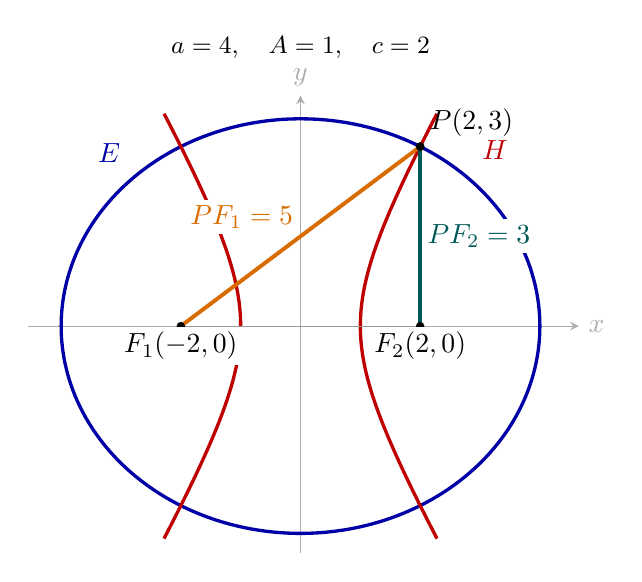
\begin{tikzpicture}[scale=0.76,>=stealth]
 \node[font=\small] at (0,4.65) {$a=4,\quad A=1,\quad c=2$};
 \draw[->,gray!65] (-4.55,0)--(4.65,0) node[right]{$x$};
 \draw[->,gray!65] (0,-3.8)--(0,3.85) node[above]{$y$};
 \draw[blue!65!black,very thick,samples=160,domain=0:360,smooth,variable=\t]
  plot ({4*cos(\t)},{sqrt(12)*sin(\t)});
 \draw[red!75!black,very thick,samples=110,domain=-3.55:3.55,variable=\t]
  plot ({sqrt(1+\t*\t/3)},{\t});
 \draw[red!75!black,very thick,samples=110,domain=-3.55:3.55,variable=\t]
  plot ({-sqrt(1+\t*\t/3)},{\t});
 \coordinate (L) at (-2,0); \coordinate (R) at (2,0); \coordinate (P) at (2,3);
 \draw[orange!85!black,line width=1.4pt] (L)--(P) node[midway,above left,fill=white,inner sep=2pt]{$PF_1=5$};
 \draw[teal!70!black,line width=1.4pt] (R)--(P) node[midway,right,fill=white,inner sep=2pt]{$PF_2=3$};
 \draw[gray!80] (L)--(R);
 \fill (L) circle (2pt) node[below,fill=white,inner sep=2pt]{$F_1(-2,0)$};
 \fill (R) circle (2pt) node[below,fill=white,inner sep=2pt]{$F_2(2,0)$};
 \fill (P) circle (2.1pt) node[above right]{$P(2,3)$};
 \node[blue!65!black] at (-3.2,2.9) {$E$};
 \node[red!75!black] at (3.25,2.95) {$H$};
\end{tikzpicture}

\end{center}
图中同一个 $P$ 同时在蓝色椭圆与红色双曲线上，
两条彩色焦半径同时受“定和”与“定差”约束。

\textbf{第1步，写定义：}设 $r_1=PF_1,r_2=PF_2$，由同一个公共点满足两条曲线的定义，
\[r_1+r_2=2a,\qquad |r_1-r_2|=2A.\]
\textbf{第2步，解和差：}较长、较短焦半径分别为
\[
\frac{(2a)+(2A)}2=a+A,\qquad
\frac{(2a)-(2A)}2=a-A.
\]
\textbf{第3步，判支别：}右支距离左焦点更远，左支距离右焦点更远，所以
\[
\boxed{\begin{array}{ll}
x_P>0:&r_1=a+A,\quad r_2=a-A,\\[2pt]
x_P<0:&r_1=a-A,\quad r_2=a+A.
\end{array}}
\]
\textbf{识别信号：}一看到“共焦＋公共点”求焦半径，先写定义，
不必先联立两条标准方程。
\end{proofbox}

\clearpage
\begin{proofbox}
\textbf{方法二：最低门槛证明（平均值＋一半差）}

\begin{center}
% C093：长度分解教学图；真实线段长度与 9:7:5:2 一致。
% 长焦半径=9=7+2，短焦半径=5=7-2。
\begin{tikzpicture}[x=0.76cm,y=0.88cm,>=stealth]
  % 平均值分界 7
  \draw[gray!65,densely dashed] (7,-0.9)--(7,2.65);
  \node[gray!70!black,above] at (7,2.65) {$a=7$};
  \node[anchor=west] at (-0.4,3.2) {\textbf{同一平均值 $7$，一长一短}};
  % Long bar 0..7 plus 7..9
  \draw[teal!70!black,line width=5pt] (0,1.9)--(7,1.9);
  \draw[orange!88!black,line width=5pt] (7,1.9)--(9,1.9);
  \draw[black,thin] (0,1.62)--(0,2.18) (9,1.62)--(9,2.18);
  \node[anchor=east] at (-0.3,1.9) {较长};
  \node[above,teal!70!black] at (3.4,1.97) {$a=7$};
  \node[above,orange!88!black] at (8.0,1.97) {$A=2$};
  \node[anchor=west] at (9.3,1.9) {$9=7+2$};
  % Short bar 0..5, dashed deficit to avg length=7
  \draw[teal!70!black,line width=5pt] (0,0.15)--(5,0.15);
  \draw[orange!85!black,densely dashed,line width=1.7pt] (5,0.15)--(7,0.15);
  \draw[black,thin] (0,-0.12)--(0,0.43) (5,-0.12)--(5,0.43);
  \node[anchor=east] at (-0.3,0.15) {较短};
  \node[above,teal!70!black] at (2.4,0.22) {$a-A=5$};
  \node[below,orange!88!black] at (6,-0.05) {少 $2$};
  \node[anchor=west] at (9.3,0.15) {$5=7-2$};
  \node[gray!75!black,anchor=west] at (0,-1.5) {实线是真实长度，虚线表示“距平均值还差 $2$”。};
\end{tikzpicture}

\end{center}

\textbf{第一步：}椭圆规定两条焦半径总长 $2a$，
所以每条长度的\emph{平均值}是 $a$。

\textbf{第二步：}双曲线规定两条长度相差 $2A$，
一条比平均值多 $A$，另一条比平均值少 $A$。
因此不论公共点在哪里，长短两条的长度都是
\[\boxed{a+A\quad\text{和}\quad a-A}.\]

\textbf{第三步：}右支点离左焦点远，把长的分配给 $PF_1$；
左支点离右焦点远，把长的分配给 $PF_2$。
也可由
\[PF_1^2-PF_2^2=4cx_P\]
检验远近。$a>c>A>0$ 保证短的一条也严格大于 $0$。

\textbf{这套方法的价值：}即使一时忘记代数加减消元，
仍可用“平均数与偏离量”重新想出公式。
\end{proofbox}

\clearpage
\begin{proofbox}
\textbf{方法三：常规坐标法（联立标准方程＋距离公式）}

\begin{center}
% Exact representative: c=3, a=5, A=2,
% P=(10/3,4sqrt(5)/3), PF1=7, PF2=3.
% Both right triangles share PQ; horizontal legs are x_P+c and x_P-c.
\begin{tikzpicture}[x=0.95cm,y=0.95cm,>=stealth,font=\small]
 \coordinate (L) at (-3,0);
 \coordinate (R) at (3,0);
 \coordinate (P) at ({10/3},{4*sqrt(5)/3});
 \coordinate (Q) at ({10/3},0);
 \draw[->,gray!65] (-3.9,0)--(4.55,0) node[right]{$x$};
 \draw[->,gray!65] (0,-0.35)--(0,3.85) node[above]{$y$};
 \draw[orange!85!black,very thick] (L)--(P)
   node[pos=0.46,above left,fill=white,inner sep=2pt]{$r_1=PF_1$};
 \draw[teal!70!black,very thick] (R)--(P)
   node[pos=0.55,right=5pt]{$r_2=PF_2$};
 \draw[densely dashed,gray!80] (P)--(Q);
 \draw[gray!80] ({10/3-0.17},0)--({10/3-0.17},0.17)--({10/3},0.17);
 \node[anchor=west] at (3.7,3.42) {$P(x_P,y_P)$};
 \node[anchor=east,fill=white,inner sep=2pt] at (2.72,1.02) {$PQ=|y_P|$};
 \draw[gray!70] (2.77,1.02)--({10/3},1.02);
 \fill (L) circle (2pt) node[below=4pt]{$F_1(-c,0)$};
 \fill (R) circle (2pt) node[below left=4pt]{$F_2(c,0)$};
 \fill (P) circle (2pt);
 \fill (Q) circle (1.6pt) node[below right=4pt]{$Q(x_P,0)$};
 \draw[<->,orange!85!black] (-3,-0.95)--({10/3},-0.95)
   node[midway,below]{$F_1Q=x_P+c$};
 \node[teal!70!black,anchor=west] at (0.4,-2.05) {$F_2Q=x_P-c$（此图 $x_P>c$）};
 \draw[teal!70!black] ({19/6},-0.1)--(4.3,-1.65)--(4.3,-1.82);
 \node[anchor=west] at (-3.6,4.55) {\textbf{两条距离共用同一高度 $PQ$}};
 \node[anchor=west] at (-3.6,-2.85) {一般情形水平距离取绝对值，平方后仍为 $(x_P\pm c)^2$。};
\end{tikzpicture}

\end{center}
过 $P$ 向 $x$ 轴作垂线，垂足为 $Q$。图中两个直角三角形
共用高度 $|y_P|$，分别给出距离平方 $(x_P+c)^2+y_P^2$、
$(x_P-c)^2+y_P^2$；一般位置的水平距离应取绝对值。

\end{proofbox}
\clearpage
\begin{proofbox}
\textbf{方法三（续）：先求坐标平方，再还原正长度。}

\textbf{第1步：}由共焦条件，写出同一个公共点的两条方程：
\[
\boxed{\frac{x^2}{a^2}+\frac{y^2}{b^2}=1},\qquad
\boxed{\frac{x^2}{A^2}-\frac{y^2}{B^2}=1},
\]
其中 $a>b>0$、$A,B>0$，且
\[\boxed{a^2-b^2=A^2+B^2=c^2}.\]
两式分别整理为
\[
 y^2=b^2\left(1-\frac{x^2}{a^2}\right),\qquad
 y^2=B^2\left(\frac{x^2}{A^2}-1\right).
\]
\textbf{第2步：}同一个公共点的纵坐标平方 $y^2$ 相同，
因此让两式相等，消去 $y^2$：
\[
 b^2+B^2=x^2\left(\frac{b^2}{a^2}+\frac{B^2}{A^2}\right).
\]
用共焦条件 $b^2=a^2-c^2$、$B^2=c^2-A^2$ 代入：
\[
 a^2-A^2
 =c^2x^2\left(\frac1{A^2}-\frac1{a^2}\right)
 =\frac{c^2x^2(a^2-A^2)}{a^2A^2}.
\]
因为 $a>c>A>0$，所以 $a^2-A^2>0$，可以约去，得到
\[
\boxed{x^2=\frac{a^2A^2}{c^2}}.
\]
将其代入椭圆方程，再利用 $c^2-A^2=B^2$，得到
\[
y^2=b^2\left(1-\frac{A^2}{c^2}\right)
=\boxed{\frac{b^2B^2}{c^2}}>0.
\]
\textbf{第3步：}由距离公式和已求得的 $x^2,y^2$，
\[
\begin{aligned}
PF_1^2&=(x+c)^2+y^2=a^2+A^2+2cx,\\
PF_2^2&=(x-c)^2+y^2=a^2+A^2-2cx.
\end{aligned}
\]
当 $x=aA/c>0$ 时，两式为
$(a+A)^2$、$(a-A)^2$；当 $x<0$ 时交换。
因为焦半径是正长度，取正平方根就得到主结论。

\textbf{方法定位：}坐标法较慢，但适合题目还要求验证公共点位置时使用；
若主要目标是求四个公共点的坐标，转入 C094。
\end{proofbox}

\clearpage
\begin{proofbox}
\textbf{补充：两点距离平方相减，快速检查左右支。}

\begin{center}
% Exact representative: c=3, a=5, A=2,
% P=(10/3,4sqrt(5)/3), PF1=7, PF2=3.
% Both right triangles share PQ; horizontal legs are x_P+c and x_P-c.
\begin{tikzpicture}[x=0.95cm,y=0.95cm,>=stealth,font=\small]
 \coordinate (L) at (-3,0);
 \coordinate (R) at (3,0);
 \coordinate (P) at ({10/3},{4*sqrt(5)/3});
 \coordinate (Q) at ({10/3},0);
 \draw[->,gray!65] (-3.9,0)--(4.55,0) node[right]{$x$};
 \draw[->,gray!65] (0,-0.35)--(0,3.85) node[above]{$y$};
 \draw[orange!85!black,very thick] (L)--(P)
   node[pos=0.46,above left,fill=white,inner sep=2pt]{$r_1=PF_1$};
 \draw[teal!70!black,very thick] (R)--(P)
   node[pos=0.55,right=5pt]{$r_2=PF_2$};
 \draw[densely dashed,gray!80] (P)--(Q);
 \draw[gray!80] ({10/3-0.17},0)--({10/3-0.17},0.17)--({10/3},0.17);
 \node[anchor=west] at (3.7,3.42) {$P(x_P,y_P)$};
 \node[anchor=east,fill=white,inner sep=2pt] at (2.72,1.02) {$PQ=|y_P|$};
 \draw[gray!70] (2.77,1.02)--({10/3},1.02);
 \fill (L) circle (2pt) node[below=4pt]{$F_1(-c,0)$};
 \fill (R) circle (2pt) node[below left=4pt]{$F_2(c,0)$};
 \fill (P) circle (2pt);
 \fill (Q) circle (1.6pt) node[below right=4pt]{$Q(x_P,0)$};
 \draw[<->,orange!85!black] (-3,-0.95)--({10/3},-0.95)
   node[midway,below]{$F_1Q=x_P+c$};
 \node[teal!70!black,anchor=west] at (0.4,-2.05) {$F_2Q=x_P-c$（此图 $x_P>c$）};
 \draw[teal!70!black] ({19/6},-0.1)--(4.3,-1.65)--(4.3,-1.82);
 \node[anchor=west] at (-3.6,4.55) {\textbf{两条距离共用同一高度 $PQ$}};
 \node[anchor=west] at (-3.6,-2.85) {一般情形水平距离取绝对值，平方后仍为 $(x_P\pm c)^2$。};
\end{tikzpicture}

\end{center}
观察共用的垂线 $PQ$：两条距离平方相减时，高度平方 $y_P^2$ 抵消。

把 $PF_1$ 和 $PF_2$ 平方相减，
\[
PF_1^2-PF_2^2=4cx_P
=(PF_1-PF_2)(PF_1+PF_2).
\]
右支 $x_P>0$，故左边大于零，$PF_1-PF_2=2A$；
左支 $x_P<0$，故左边小于零，$PF_1-PF_2=-2A$。
利用 $PF_1+PF_2=2a$，两个支别的公式便得到独立核查。

\textbf{关键意义：}相减不是机械消元；它让两次出现的 $y_P^2$
消失，直接读出点在左侧还是右侧。若只为求焦半径，
无需进一步求交点坐标。
\end{proofbox}

\clearpage
\begin{examplebox}
\textbf{例1（母题：标准方程直接求焦半径）。}

已知
\[
E:\ \frac{x^2}{16}+\frac{y^2}{12}=1,\qquad
H:\ x^2-\frac{y^2}{3}=1.
\]
$P$ 是两条曲线第一象限的公共点。求 $PF_1$、$PF_2$。

\begin{center}
% C093: a=4, A=1, c=2; E: x^2/16+y^2/12=1, H: x^2-y^2/3=1
% Intersection P=(2,3); PF1=5, PF2=3; generated as exact coordinate constructions.
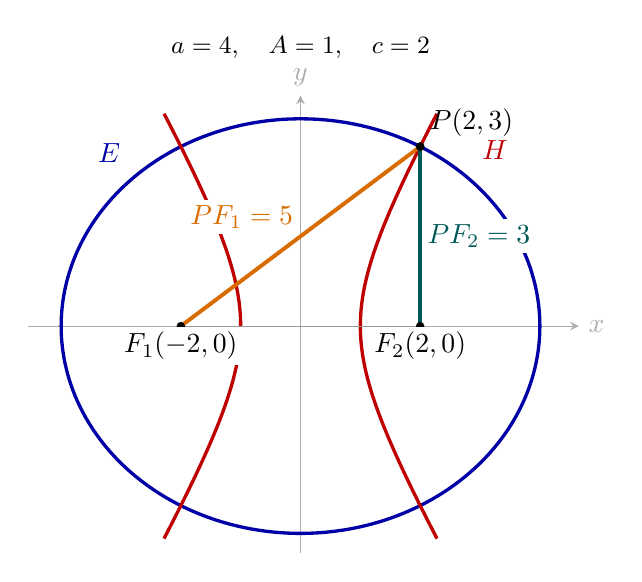
\begin{tikzpicture}[scale=0.76,>=stealth]
 \node[font=\small] at (0,4.65) {$a=4,\quad A=1,\quad c=2$};
 \draw[->,gray!65] (-4.55,0)--(4.65,0) node[right]{$x$};
 \draw[->,gray!65] (0,-3.8)--(0,3.85) node[above]{$y$};
 \draw[blue!65!black,very thick,samples=160,domain=0:360,smooth,variable=\t]
  plot ({4*cos(\t)},{sqrt(12)*sin(\t)});
 \draw[red!75!black,very thick,samples=110,domain=-3.55:3.55,variable=\t]
  plot ({sqrt(1+\t*\t/3)},{\t});
 \draw[red!75!black,very thick,samples=110,domain=-3.55:3.55,variable=\t]
  plot ({-sqrt(1+\t*\t/3)},{\t});
 \coordinate (L) at (-2,0); \coordinate (R) at (2,0); \coordinate (P) at (2,3);
 \draw[orange!85!black,line width=1.4pt] (L)--(P) node[midway,above left,fill=white,inner sep=2pt]{$PF_1=5$};
 \draw[teal!70!black,line width=1.4pt] (R)--(P) node[midway,right,fill=white,inner sep=2pt]{$PF_2=3$};
 \draw[gray!80] (L)--(R);
 \fill (L) circle (2pt) node[below,fill=white,inner sep=2pt]{$F_1(-2,0)$};
 \fill (R) circle (2pt) node[below,fill=white,inner sep=2pt]{$F_2(2,0)$};
 \fill (P) circle (2.1pt) node[above right]{$P(2,3)$};
 \node[blue!65!black] at (-3.2,2.9) {$E$};
 \node[red!75!black] at (3.25,2.95) {$H$};
\end{tikzpicture}

\end{center}

\textbf{识别：}给出两条标准方程，先核查是否共焦，再使用定和、定差。

\textbf{解：}椭圆 $a=4$、$b^2=12$，所以 $c^2=a^2-b^2=16-12=4$；
双曲线 $A=1$、$B^2=3$，所以 $c^2=A^2+B^2=1+3=4$。
两条曲线的焦点确为 $F_1=(-2,0)$、$F_2=(2,0)$。
$P$ 在第一象限，横坐标大于零，属于双曲线右支，所以
\[
\boxed{PF_1=4+1=5,\qquad PF_2=4-1=3}.
\]
\textbf{回验：}$PF_1+PF_2=8=2a$，
$PF_1-PF_2=2=2A$；
这里\emph{无需先求 $P$ 的坐标}。
\end{examplebox}

\clearpage
\begin{examplebox}
\textbf{例2（变式：仅给离心率，并比较左右支）。}

椭圆与双曲线共焦，焦距 $F_1F_2=6$，
椭圆离心率 $e_1=\frac35$，双曲线离心率 $e_2=\frac32$。
$P$ 为第二象限公共点，$Q$ 为第一象限公共点。
分别求 $PF_1,PF_2,QF_1,QF_2$。

\textbf{识别：}给离心率先求半轴；象限直接告诉我们支别。

\textbf{解：}$c=3$，故
\[
a=\frac{3}{3/5}=5,\qquad A=\frac{3}{3/2}=2.
\]
较长的焦半径为 $7$，较短的为 $3$。
$P$ 在左支，离 $F_1$ 较近；$Q$ 在右支，离 $F_2$ 较近。因此
\[
\boxed{PF_1=3,\quad PF_2=7;\qquad QF_1=7,\quad QF_2=3}.
\]
\textbf{回验：}两点的焦半径和都为 $10$，差的绝对值都为 $4$。
\textbf{最小反例：}若给左支点写 $PF_1=7>PF_2=3$，
则与 $PF_1^2-PF_2^2=4cx_P<0$ 矛盾。
\end{examplebox}

\clearpage
\begin{examplebox}
\textbf{例3（反向题：由焦半径还原两条曲线）。}

$F_1=(-4,0)$、$F_2=(4,0)$ 是共焦椭圆与双曲线的焦点。
右支公共点 $P$ 满足 $PF_1=9$、$PF_2=5$。
求椭圆与双曲线的标准方程。

\textbf{识别：}给两条焦半径，反过来使用定和、定差求半轴。

\textbf{解：}由椭圆与双曲线定义，
\[
a=\frac{9+5}{2}=7,\qquad A=\frac{9-5}{2}=2,\qquad c=4.
\]
椭圆半短轴平方 $b^2=a^2-c^2=49-16=33$；
双曲线虚半轴平方 $B^2=c^2-A^2=16-4=12$。
因此
\[
\boxed{E:\ \frac{x^2}{49}+\frac{y^2}{33}=1},\qquad
\boxed{H:\ \frac{x^2}{4}-\frac{y^2}{12}=1}.
\]
\textbf{回验：}$7>4>2>0$，参数满足共焦条件；
$2a=14=9+5$，$2A=4=9-5$。

\textbf{延伸：}若题目要求列出四个公共点及坐标，
可用 C094 的交点坐标方法继续求解，不必在 C093 重做整套推导。
\end{examplebox}

\clearpage
\begin{trapbox}
\textbf{易错点1：左右支把两个焦半径分配反了。}

\begin{center}
% C093：左右同尺度的错误/正确配对对照；几何长度始终为3和5。
% 公共点位于左支，F1=(0,0),F2=(4,0),P=(0,3) (局部平移坐标)
\begin{tikzpicture}[scale=0.82,>=stealth]
 \begin{scope}
  \coordinate (L) at (0,0); \coordinate (R) at (4,0); \coordinate (P) at (0,3);
  \draw[gray,thick] (L)--(R);
  \draw[teal!70!black,very thick] (L)--(P);
  \draw[orange!85!black,very thick] (R)--(P);
  \foreach \q/\loc/\t in {L/below/F_1,R/below/F_2,P/above/P}{\fill (\q) circle(1.8pt) node[\loc]{$\t$};}
  \node[red!75!black,above] at (2,3.65) {\textbf{错误：数值配反}};
  \node[red!75!black,left] at (-0.08,1.5) {$PF_1=5\;\times$};
  \node[red!75!black,above right] at (2.2,1.8) {$PF_2=3\;\times$};
  \node[below] at (2,-0.85) {$P$ 在左支，近 $F_1$};
 \end{scope}
 \begin{scope}[xshift=7cm]
  \coordinate (L) at (0,0); \coordinate (R) at (4,0); \coordinate (P) at (0,3);
  \draw[gray,thick] (L)--(R);
  \draw[teal!70!black,very thick] (L)--(P);
  \draw[orange!85!black,very thick] (R)--(P);
  \foreach \q/\loc/\t in {L/below/F_1,R/below/F_2,P/above/P}{\fill (\q) circle(1.8pt) node[\loc]{$\t$};}
  \node[teal!70!black,above] at (2,3.65) {\textbf{正确：按实际长度}};
  \node[teal!70!black,left] at (-0.08,1.5) {$PF_1=3$};
  \node[orange!85!black,above right] at (2.2,1.8) {$PF_2=5$};
  \node[below] at (2,-0.85) {$3^2-5^2<0$};
 \end{scope}
\end{tikzpicture}

\end{center}

左支的点离左焦点近，离右焦点远。
图中两幅三角形\emph{点的位置和实际长度相同}，
左图故意把 $3$、$5$ 标签写反，以便和右图逐一对照。
\[
\boxed{x_P<0\ \Longrightarrow\ PF_1<PF_2},\qquad
PF_1^2-PF_2^2=4cx_P<0.
\]
\textbf{正确替代：}先写无序的 $\{a+A,a-A\}$，
再看点在左支还是右支，最后决定哪段对应哪个焦点。
\end{trapbox}

\clearpage
\begin{trapbox}
\textbf{其他易错点：错误写法 $\to$ 错因 $\to$ 正确做法。}
\begin{itemize}
\item \textbf{漏掉绝对值：}误写
$PF_1-PF_2=2A$ 适用于所有公共点。
左支的差是负数；应写
$|PF_1-PF_2|=2A$，再按支别确定符号。
例如 $F_1=(-2,0),F_2=(2,0),P=(-2,3)$ 时，
$PF_1-PF_2=3-5=-2$。

\item \textbf{半轴混淆或再乘2：}若 $a=4,A=1$，
正确两长度为 $5,3$；写成 $10,6$ 是把已经求出的长度重复乘2。
必须区分 $a$ 与 $A$，共焦\emph{只表示焦点相同}。

\item \textbf{把两条曲线不同的点联立：}若一个点在椭圆、另一个点在双曲线，
不能把两个点各自满足的关系写成同一个方程组。
必须先确认是\emph{同一个公共点}、\emph{同一对焦点}。

\item \textbf{忽略参数范围：}写出 $a-A$ 前应核对
$a>c>A>0$；例如 $c=2,A=4$ 就不满足双曲线的焦距关系。
两条焦半径必须为正长度。
\end{itemize}
\end{trapbox}

\clearpage
\begin{trapbox}
\textbf{易错点：误以为上下对称也会交换两条焦半径。}

\begin{center}
% Four exact intersections for a=4, A=1, c=2: (+/-2,+/-3)
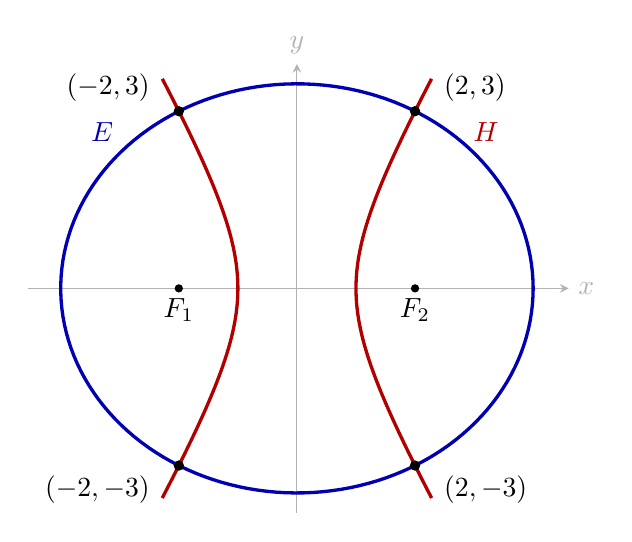
\begin{tikzpicture}[scale=0.75,>=stealth]
 \draw[->,gray!60] (-4.55,0)--(4.6,0) node[right]{$x$};
 \draw[->,gray!60] (0,-3.8)--(0,3.8) node[above]{$y$};
 \draw[blue!70!black,very thick,samples=160,domain=0:360,variable=\t]
  plot ({4*cos(\t)},{sqrt(12)*sin(\t)});
 \draw[red!70!black,very thick,samples=110,domain=-3.55:3.55,variable=\t]
  plot ({sqrt(1+\t*\t/3)},{\t});
 \draw[red!70!black,very thick,samples=110,domain=-3.55:3.55,variable=\t]
  plot ({-sqrt(1+\t*\t/3)},{\t});
 \foreach \x/\y in {2/3,2/-3,-2/3,-2/-3}{\fill[black] (\x,\y) circle (2.5pt);}
 \node[above right,xshift=7pt] at (2,3) {$(2,3)$};
 \node[below right,xshift=7pt] at (2,-3) {$(2,-3)$};
 \node[above left,xshift=-7pt] at (-2,3) {$(-2,3)$};
 \node[below left,xshift=-7pt] at (-2,-3) {$(-2,-3)$};
 \fill (-2,0) circle (2pt) node[below]{$F_1$};
 \fill (2,0) circle (2pt) node[below]{$F_2$};
 \node[blue!70!black] at (-3.3,2.65) {$E$};
 \node[red!70!black] at (3.2,2.65) {$H$};
\end{tikzpicture}

\end{center}

图中右侧 $(2,3)$ 与 $(2,-3)$ 关于 $x$ 轴对称，
到 $F_1$ 的距离同为 $5$，到 $F_2$ 的距离同为 $3$；
左侧两点则到 $F_1$ 同为 $3$、到 $F_2$ 同为 $5$。
\textbf{正确替代：}上下对称保持到每个焦点的距离；
只有左右对称才交换焦点对应。判长短看 $x_P$ 的正负。
\end{trapbox}

\clearpage
\begin{trapbox}
\textbf{三个15秒自测（可直接当课堂提问）。}
\begin{enumerate}
\item $a=6,A=2$，点在左支，求 $PF_1,PF_2$。
\textbf{答：}$PF_1=4,PF_2=8$。
\item $PF_1=8,PF_2=4$，反求 $a,A$。
\textbf{答：}$a=6,A=2$。
\item 焦距 $6$，椭圆半长轴 $5$、双曲线实半轴 $2$；
右支公共点到哪个焦点更近？
\textbf{答：}到右焦点 $F_2$ 更近，$PF_2=3$。
\end{enumerate}
\textbf{检查顺序：}共同焦点与同一个公共点 $\to$ 半轴范围
$\to$ 定和定差 $\to$ 左右支 $\to$ 正长度。
\end{trapbox}

\clearpage
\begin{summarybox}
\textbf{C093\quad 共焦椭圆与双曲线公共点的焦半径公式：快记／快懂／快用}

\textbf{快记（一组长度，两种对应）：}
\[
\boxed{\{PF_1,PF_2\}=\{a+A,\ a-A\}},\qquad a>c>A>0.
\]
\[
\boxed{\begin{array}{ll}
\text{右支 }x_P>0:&PF_1=a+A,\quad PF_2=a-A,\\[2pt]
\text{左支 }x_P<0:&PF_1=a-A,\quad PF_2=a+A.
\end{array}}
\]

\textbf{快懂（和、差决定两条长度）：}
\[
\underbrace{PF_1+PF_2=2a}_{\text{椭圆：总长}},\qquad
\underbrace{|PF_1-PF_2|=2A}_{\text{双曲线：长度差}}.
\]
两条长度的平均值是 $a$，各自离平均值相差 $A$。

\textbf{快用（三步）：}
\begin{enumerate}
\item 确认\emph{同一对焦点、同一个公共点}，且 $a>c>A>0$；
\item 直接求\emph{较长} $a+A$ 与\emph{较短} $a-A$；
\item 看横坐标正负：\emph{右支左焦点远，左支右焦点远}。
\end{enumerate}

\textbf{离心率速换：}
\[
a=\frac c{e_1},\qquad A=\frac c{e_2},\qquad
\{PF_1,PF_2\}=\left\{c\left(\frac1{e_1}+\frac1{e_2}\right),
 c\left(\frac1{e_1}-\frac1{e_2}\right)\right\}.
\]
\textbf{最后检查：}差式别漏绝对值；两种半轴别混用；
没给支别就别给 $PF_1,PF_2$ 强行排序。

\textbf{一句话：}椭圆给和，双曲线给差；先算长短，再分左右。
\end{summarybox}

